\documentclass[12pt,aps,pre]{revtex4}
%\documentclass[aps,pre,onecolumn,superscriptaddress]{revtex4-1}
\usepackage{graphicx, epsfig,cancel}
\usepackage{color}
\usepackage{textcomp}
\usepackage{amssymb,amsmath} 
\usepackage{setspace}

% for writing code snippets in latex
\usepackage{listings}

\definecolor{dkgreen}{rgb}{0,0.6,0}
\definecolor{gray}{rgb}{0.5,0.5,0.5}
\definecolor{mauve}{rgb}{0.58,0,0.82}

\lstset{frame=tb,
  language=C++,
  aboveskip=3mm,
  belowskip=3mm,
  showstringspaces=false,
  columns=flexible,
  basicstyle={\small\ttfamily},
  numbers=none,
  numberstyle=\tiny\color{gray},
  keywordstyle=\color{blue},
  commentstyle=\color{dkgreen},
  stringstyle=\color{mauve},
  breaklines=true,
  breakatwhitespace=true,
  tabsize=3
}

\newcommand{\blue}[1]{\textcolor{blue}{#1}}
\newcommand{\red}[1]{\textcolor{red}{[#1]}}
\newcommand{\green}[1]{\textcolor{green}{#1}}

\begin{document}
\setstretch{1.5}
\title{Multi-Scale Formulation for Biotissue Code}
\author{V. W. L. Chan}
\maketitle

\section{Macro-scale}

\subsection{Governing Equation}

The divergence of the macroscopic stress tensor, $\pmb{\sigma}$ is derived by applying the Reynolds transport theorem to the volume-averaged stress and invoking microscopic equilibrium \cite{Chandran:2007hy,Stylianopoulos:2007dp} 
%
\begin{equation}
\sigma_{ij,i}^{(M)} = \frac{1}{V^{(m)}} \int_{\partial V^{(m)}} \left( s_{ij}^{(m)} - \sigma_{ij}^{(M)} \right)u_{k,i}^{(m)} n_k dA^{(m)},
\label{eq:macro_stress_divergence}
\end{equation}
%
where $u_k^{(m)}$ is the displacement of the RVE boundary on the microscale (right superscript $(m)$), $n_k$ is the unit normal vector, and $s_{ij}^{(m)}$ are elements of the microscopic stress tensor. A volume averaging of $s_{ij}^{(m)}$ is employed to obtain $\sigma_{ij}^{(M)}$ \cite{Chandran:2007hy}:
%
\begin{equation}
\sigma_{ij}^{(M)} = \frac{1}{V^{(m)}}\int_{V^{(m)}}s_{ij}^{(m)} dV^{(m)},
\label{eq:macro_stress_volume_avg}
\end{equation}
%
where $V^{(m)}$ is the microscale volume.

The virtual work, $\delta W$, is obtained by multiplying Eq.\ \eqref{eq:macro_stress_divergence} by multiplying by a virtual velocity, $\delta \pmb{v}$ (also known as a test function), and integrating over the current volume \cite{JavierBonet:2008uxa}
%
\begin{align}
\delta W &= \int_{V^{(M)}} \left(\sigma_{ij,i}^{(M)} - \frac{1}{V^{(m)}} \int_{\partial V^{(m)}} \left( s_{ij}^{(m)} - \sigma_{ij}^{(M)} \right)u_{k,i}^{(m)} n_k dA^{(m)} \right)  \delta v_j^{(M)}  dV^{(M)} \nonumber\\
%
&= \int_{V_0^{(M)}} \left(\sigma_{ij,i}^{(M)} - \frac{1}{V^{(m)}} \int_{\partial V^{(m)}} \left( s_{ij}^{(m)} - \sigma_{ij}^{(M)} \right)u_{k,i}^{(m)} n_k dA^{(m)} \right)  \delta v_j^{(M)}J dV_0^{(M)}  \nonumber\\
%
&= \int_{V_0^{(M)}} \left(\sigma_{ij,i}^{(M)} - Q_j^{(m/M)} \right) \delta v_j^{(M)}J dV_0^{(M)}   \nonumber\\
%
&= \int_{V_0^{(M)}} \left(\text{div}\pmb{\sigma}^{(M)} - \pmb{Q}^{(m/M)} \right)  \cdot \delta \pmb{v}^{(M)}J dV_0^{(M)} ,
\label{eq:virtual_work}
\end{align}
%
where  
%
\begin{equation}
Q_j^{(m/M)} = \frac{1}{V^{(m)}} \int_{\partial V^{(m)}} \left( s_{ij}^{(m)} - \sigma_{ij}^{(M)} \right)u_{k,i}^{(m)} n_k dA^{(m)}.
\end{equation}
%
Note that the superscript $(m/M)$ indicates the quantity involves variables from both the micro and macro scales. 

Using the identity
%
\begin{equation}
\text{div}(\pmb{\sigma}\delta\pmb{v} J) =  (\pmb{\sigma}:\delta\pmb{v})J + (\delta \pmb{v} \cdot \text{div}\pmb{\sigma})J + (\pmb{\sigma} \delta\pmb{v})\cdot \nabla J
\end{equation}
%
Eq.\ \eqref{eq:virtual_work} becomes
%
\begin{eqnarray}
\delta W &=& \int_{V_0^{(M)}} \left(\text{div}(\pmb{\sigma}^{(M)} \delta\pmb{v}^{(M)} J) - (\pmb{\sigma}^{(M)}:\nabla \delta \pmb{v}) J - (\pmb{\sigma}^{(M)}\delta \pmb{v}^{(M)})\cdot \nabla J \right)dV_0^{(M)} \nonumber\\
%
&-& \int_{V_0^{(M)}} \pmb{Q}^{(m/M)} \cdot \delta \pmb{v}^{(M)}J dV_0^{(M)} 
%
\end{eqnarray}
%
Further applying the divergence theorem we have
%
\begin{eqnarray}
\delta W &=& \int_{\partial V_0^{(M)}} \pmb{n} \cdot \pmb{\sigma}^{(M)} \delta\pmb{v}^{(M)} J dA_0^{(M)} - \int_{V_0^{(M)}} \left((\pmb{\sigma}^{(M)}:\nabla \delta \pmb{v}) J + (\pmb{\sigma}^{(M)}\delta \pmb{v}^{(M)})\cdot \nabla J \right)dV_0^{(M)} \nonumber\\
%
&-& \int_{V_0^{(M)}} \pmb{Q}^{(m/M)} \cdot \delta \pmb{v}^{(M)}J dV_0^{(M)} \nonumber\\
%
&=& \int_{\partial V_0^{(M)}} \pmb{t}^{(M)} \cdot \delta\pmb{v}^{(M)} J dA_0^{(M)} - \int_{V_0^{(M)}} \left((\pmb{\sigma}^{(M)}:\nabla \delta \pmb{v}) J + (\pmb{\sigma}^{(M)}\delta \pmb{v}^{(M)})\cdot \nabla J \right)dV_0^{(M)} \nonumber\\
%
&-& \int_{V_0^{(M)}} \pmb{Q}^{(m/M)} \cdot \delta \pmb{v}^{(M)}J dV_0^{(M)} \nonumber\\
&=& \int_{V_0^{(M)}} \left((\pmb{\sigma}^{(M)}:\delta \pmb{d}) J + (\pmb{\sigma}^{(M)}\delta \pmb{v}^{(M)})\cdot \nabla J \right)dV_0^{(M)} \nonumber\\
%
&-& \int_{\partial V_0^{(M)}} \pmb{t}^{(M)} \cdot \delta\pmb{v}^{(M)} J dA_0^{(M)} + \int_{V_0^{(M)}} \pmb{Q}^{(m/M)} \cdot \delta \pmb{v}^{(M)}J dV_0^{(M)} \nonumber\\
%
&=& \delta W_{int} + \delta W_{ext}
\label{eq:virtual_work_final}
\end{eqnarray}
%
where $\delta \pmb{d}^{(M)}$ is the virtual rate of deformation tensor and $\pmb{t}^{(M)}$ is the traction vector.

\subsection{Newton-Raphson Method and the Tangent-Stiffness Matrix}

The Newton-Raphson procedure for solving a nonlinear set of equations is \cite{JavierBonet:2008uxa}
%
\begin{eqnarray}
\pmb{K}(\pmb{u}^k) \delta \pmb{u} = - \pmb{R}(\pmb{u}^k), \ \pmb{u}^{k+1} = \pmb{u}^k + \delta \pmb{u},
\label{eq:Newton-Raphson}
\end{eqnarray}
%
where $\pmb{R}$ is the out-of-balance force, $\pmb{K}$ is the tangent stiffness matrix, and the superscript $k$ indicates the pseudo time step of the procedure. The left-hand-side of  Eq.\ \eqref{eq:Newton-Raphson} is determined from the directional derivative of $\pmb{R}$ with respect to $\pmb{u}^k$ and in the direction of $\delta \pmb{u}$:
%
\begin{eqnarray}
\pmb{K}(\pmb{u}^k) \delta \pmb{u} &=& D\pmb{R}(\pmb{u}^k)[\delta \pmb{u}] \nonumber\\
%
&=& \frac{d}{d\epsilon} \bigg|_{\epsilon=0}\pmb{R}(\pmb{u}^k + \epsilon \delta \pmb{u}) \nonumber\\
&=& \frac{d \pmb{R}}{d\pmb{u}^k} \frac{d(\pmb{u}^k + \epsilon \delta \pmb{u})}{d\epsilon} \bigg|_{\epsilon=0} \nonumber\\
&=& \frac{d \pmb{R}}{d\pmb{u}^k} \delta \pmb{u}.
\label{eq:DR[u]}
\end{eqnarray}
%
In matrix form we have
%
\begin{eqnarray}
[\pmb{K}(\pmb{u}^k)][\delta \pmb{u}] =
%
\begin{bmatrix}
\frac{\partial R_1}{\partial u_1^k} & \frac{\partial R_1}{\partial u_2^k} & \frac{\partial R_1}{\partial u_3^k} \\
%
\frac{\partial R_2}{\partial u_1^k} & \frac{\partial R_2}{\partial u_2^k} & \frac{\partial R_2}{\partial u_3^k} \\
%
\frac{\partial R_3}{\partial u_1^k} & \frac{\partial R_3}{\partial u_2^k} & \frac{\partial R_3}{\partial u_3^k} \\
\end{bmatrix}
%
\begin{bmatrix}
\delta u_1 \\ \delta u_2 \\ \delta u_3
\end{bmatrix}, \ \ \text{where} \ \ 
%
[\pmb{R}] = 
\begin{bmatrix}
R_1 \\ R_2 \\ R_3
\end{bmatrix}.
\label{eq:DR[u]_matrix}
\end{eqnarray}
%

To apply the Newton-Raphson procedure to our problem, the virtual work in Eq.\ \eqref{eq:virtual_work} must be linearized by taking the directional derivative of $\delta W$ with respect to $\delta \pmb{v}$ in the direction of $\delta \pmb{u}$ at the configuration $\phi$
%
\begin{equation}
D\delta W (\phi,\delta \pmb{v}) [\delta \pmb{u}] = D\delta W_{int} (\phi,\delta \pmb{v}) [\delta \pmb{u}] - D\delta W_{ext} (\phi,\delta \pmb{v}) [\delta \pmb{u}].
\end{equation}
%
%Since the virtual work is expressed in the current configuration (c.f., Eq.\ \eqref{eq:virtual_work}), linearization is not straightforward because the integration bound changes with motion. Therefore, to move forward with the linearization procedure, we must first linearize the virtual work expressed in the reference configuration and then  employ a push-forward operation to obtain the linearization for the spatial description of Eq.\ \eqref{eq:virtual_work}.
%
\red{$\pmb{t}$ and $\pmb{Q}$ in Eq.\ \eqref{eq:virtual_work_final} are assumed to be constant. Therefore, from this point on, only the linearization of internal virtual work, $\delta W_{int}$, is considered.} 

Up to this point I have found that the linearization of Eq.\ \eqref{eq:virtual_work_final} does not yield what is currently implemented in the biotissue code. To move forward with the implementation of using the deformation gradient tensor at the microscale, I will simply present the equations that is currently implemented in the biotissue code.

The linearized virtual work in the biotissue code is
%% begin comment
%
\begin{eqnarray}
D\delta W(\phi,\delta \pmb{v}^{(M)})[\delta \pmb{u}^{(M)}]  
%
&=& \int_V^{(M)} \left(\delta d_{ij}^{(M)} c_{ijkl}^{(M)} \varepsilon_{kl}^{(M)} +  \sigma_{ij}^{(M)} \frac{\partial \delta u_j^{(M)}}{\partial x_i^{(M)}}\frac{\partial \delta v_i^{(M)}}{\partial x_j^{(M)}}\right) d V - \int_{\partial V^{(M)}} t_i^{(M)} \delta v_i^{(M)} dA^{(M)} \nonumber\\
&-& Q_i^{(M)} \delta v_j^{(M)},
\label{eq:virtual_work_linearized}
\end{eqnarray}
%
where $\pmb{e}$ and $\pmb{\varepsilon}$ are the Eulerian (or Almansi) strain tensor and small-strain tensor, respectively, and $\delta \pmb{d}$ is the virtual rate of deformation tensor:
%
\begin{align}
&\pmb{e} = \frac{1}{2}(\pmb{I} - \pmb{b}^{-1}) \nonumber\\
%
&\pmb{\varepsilon} = \frac{1}{2}\left(\nabla \pmb{u} + (\nabla \pmb{u})^T\right) \nonumber\\
%
&\pmb{b} = \pmb{F}\pmb{F}^T \\
%
&\delta \pmb{d} = \frac{1}{2}\left(\nabla \delta \pmb{v}  + (\nabla \delta \pmb{v})^T\right).
\end{align}
%

The linearization in Eq.\ \eqref{eq:virtual_work_linearized} can be cast into the framework of the Newton-Raphson procedure in Eq.\ \eqref{eq:Newton-Raphson} by discretization via shape functions:
%
\begin{align}
&\delta \pmb{u}^{(M)} = \sum_{a=1}^n N_a \pmb{x}_a^{(M)} \nonumber\\
%
&\delta \pmb{v}^{(M)} = \sum_{a=1}^n N_a \delta \pmb{v}_a^{(M)} \nonumber\\
%
&\delta \pmb{d}^{(M)} = \frac{1}{2} \sum_{a=1}^n (\delta \pmb{v}_a^{(M)} \otimes \nabla N_a + \nabla N_a \otimes \delta \pmb{v}_a^{(M)}) \nonumber\\
%
&\delta \pmb{\varepsilon}^{(M)} = \frac{1}{2} \sum_{a=1}^n (\pmb{u}_a^{(M)} \otimes \nabla N_a + \nabla N_a \otimes \pmb{u}_a^{(M)}),
\label{eq:discretization}
\end{align}
%
where $N_a$ is the $a^{th}$ node of the shape function and $n$ is the number of nodes contained in each shape function. The discretized form of Eq.\ \eqref{eq:virtual_work_linearized} is obtained by applying the approximations in Eq.\ \eqref{eq:discretization}
%
\begin{eqnarray}
D\delta W(\phi,N_a\delta \pmb{v}_a^{(M)})[N_b\delta \pmb{u}_b^{(M)}] &=& \delta v_i^{(M),a}\left(\int_{V^{(e)}}\frac{\partial N_a}{\partial x_j^{(M)}} c_{ijkl}^{(M)} \frac{\partial N_b}{\partial x_l^{(M)}} dV^{(e)} \right) \delta u_k^{(M),b} 
\end{eqnarray}
%

In the multiscale formulation, the Cauchy stresses and their derivatives in Eq.\ \eqref{eq:virtual_work_linearized}:
%
\begin{equation}
\sigma_{ij} \ \text{and} \ \frac{\partial \sigma_{ij}}{\partial e_{kl}},
\label{eq:sigma_terms}
\end{equation}
%
are evaluated from calculations at the microscale representative volume elements (RVEs). In order to write the stress derivative in matrix form, Voigt notation is used 
%
\begin{eqnarray}
[\sigma_{(i)}] \equiv 
\begin{bmatrix}
\sigma_{11} \\ \sigma_{22} \\ \sigma_{33} \\ \sigma_{12} \\ \sigma_{23} \\ \sigma_{13}
\end{bmatrix} , \ \
%
[e_{(i)}] \equiv
\begin{bmatrix}
e_{11} \\ e_{22} \\ e_{33} \\ e_{12} \\ e_{23} \\ e_{13} 
\end{bmatrix}, \ \text{and} \
%
\left[ \frac{\partial \sigma_{(i)}}{\partial e_{(j)}} \right] \equiv 
\begin{bmatrix}
\frac{\partial \sigma_{11}}{\partial e_{11}} & \frac{\partial \sigma_{11}}{\partial e_{22}} & \frac{\partial \sigma_{11}}{\partial e_{33}} & \frac{\partial \sigma_{11}}{\partial e_{12}} & \frac{\partial \sigma_{11}}{\partial e_{23}} & \frac{\partial \sigma_{11}}{\partial e_{13}} \\
%
\frac{\partial \sigma_{22}}{\partial e_{11}} & \frac{\partial \sigma_{22}}{\partial e_{22}} & \frac{\partial \sigma_{22}}{\partial e_{33}} & \frac{\partial \sigma_{22}}{\partial e_{12}} & \frac{\partial \sigma_{22}}{\partial e_{23}} & \frac{\partial \sigma_{22}}{\partial e_{13}} \\
%
\frac{\partial \sigma_{33}}{\partial e_{11}} & \frac{\partial \sigma_{33}}{\partial e_{22}} & \frac{\partial \sigma_{33}}{\partial e_{33}} & \frac{\partial \sigma_{33}}{\partial e_{12}} & \frac{\partial \sigma_{33}}{\partial e_{23}} & \frac{\partial \sigma_{33}}{\partial e_{13}} \\
%
\frac{\partial \sigma_{12}}{\partial e_{11}} & \frac{\partial \sigma_{12}}{\partial e_{22}} & \frac{\partial \sigma_{12}}{\partial e_{33}} & \frac{\partial \sigma_{12}}{\partial e_{12}} & \frac{\partial \sigma_{12}}{\partial e_{23}} & \frac{\partial \sigma_{12}}{\partial e_{13}} \\
%
\frac{\partial \sigma_{23}}{\partial e_{11}} & \frac{\partial \sigma_{23}}{\partial e_{22}} & \frac{\partial \sigma_{23}}{\partial e_{33}} & \frac{\partial \sigma_{23}}{\partial e_{12}} & \frac{\partial \sigma_{23}}{\partial e_{23}} & \frac{\partial \sigma_{23}}{\partial e_{13}} \\
%
\frac{\partial \sigma_{13}}{\partial e_{11}} & \frac{\partial \sigma_{13}}{\partial e_{22}} & \frac{\partial \sigma_{13}}{\partial e_{33}} & \frac{\partial \sigma_{13}}{\partial e_{12}} & \frac{\partial \sigma_{13}}{\partial e_{23}} & \frac{\partial \sigma_{13}}{\partial e_{13}} 
\end{bmatrix},
\label{eq:sigma_terms_Voigt}
\end{eqnarray}
%
where the parenthesis around the subscripts indicate the use of Voigt notation.
% end comment








% begin comment
%The virtual work can be expressed in the reference configuration as 
%
%\begin{equation}
%\delta W_{int}(\phi,\delta \pmb{v}) = \int_{V_0} \pmb{S}:\delta \dot{\pmb{E}} dV_0,
%\label{eq:internal_virtual_work_reference}
%\end{equation}
%%
%where $\pmb{S}$ and $\delta \dot{\pmb{E}}$ are the second Piola-Kirchhoff stress tensor and the virtual material strain rate tensor, respectively. The virtual material strain rate tensor is 
%%
%\begin{equation}
%\delta \dot{\pmb{E}} = \frac{1}{2} (\delta \dot{\pmb{F}}^T \pmb{F} + \pmb{F}^T \dot{\pmb{F}}).
%\end{equation}
%%
%Now that the bound of the integral in Eq.\ \eqref{eq:internal_virtual_work_reference} does not change, the linearization can be determined from the directional derivative as
%%
%\begin{eqnarray}
%D\delta W_{int} (\phi,\delta \pmb{v}) [\delta \pmb{u}] &=& \int_{V_0} D(\delta \dot{\pmb{E}} : \pmb{S}[\pmb{u}] dV_0 \nonumber\\
%%
%&=& \int_{V_0} \delta \dot{\pmb{E}} : D\pmb{S}[\pmb{u}] dV_0 + \int_{V_0} \pmb{S}:D\delta \dot{\pmb{E}}[\pmb{u}] dV_0 \nonumber\\
%%
%&=& \int_{V_0} \delta \dot{E}_{ij} \frac{\partial S_{ij}}{\partial E_{kl}} DE_{kl}[\pmb{u}] dV_0 + \int_{V_0} S_{ij} \frac{\partial u_j}{\partial X_i} \frac{\partial \delta v_i}{\partial X_j} dV_0 \nonumber\\
%%
%&=&\int_{V_0} D E_{ij} [\delta \pmb{v}] \frac{\partial S_{ij}}{\partial E_{kl}} DE_{kl}[\pmb{u}] dV_0 + \int_{V_0} S_{ij} \frac{\partial u_j}{\partial X_i} \frac{\partial \delta v_i}{\partial X_j} dV_0,
%\label{eq:internal_virtal_work_reference_linearized}
%\end{eqnarray}
%% 
%where the following relationships have been used
%%
%\begin{align}
%&\delta \dot{\pmb{E}} = D \pmb{E} [\delta \pmb{v}] \nonumber\\
%%
%&DS_{ij}[\pmb{u}] = \sum_{k,l=1}^3 \frac{\partial S_{ij}}{\partial E_{kl}}DE_{kl}[\pmb{u}] .
%\end{align}
%%
%
%To arrive at the linearization for the internal virtual work in the current configuration, the following pull-back and push-forward operations are used
%%
%\begin{align}
%&D\pmb{E}[\delta \pmb{v}] = \pmb{F}^T \varepsilon \pmb{F}; \ \ \pmb{\varepsilon} = \frac{1}{2}\left(\nabla \pmb{u} + (\nabla \pmb{u})^T\right) \nonumber\\
%%
%& D\pmb{E}[\pmb{u}] = \pmb{F}^T \delta \pmb{d} \pmb{F}; \ \ \delta \pmb{d} = \frac{1}{2}\left(\nabla \delta \pmb{v}  + (\nabla \delta \pmb{v})^T\right) \nonumber\\
%%
%&\pmb{S} = J \pmb{F}^{-1} \pmb{\sigma} \pmb{F}^{-T} \nonumber\\
%%
%&\pmb{E} = \pmb{F}^T \pmb{e} \pmb{F}; \ \ \pmb{e} = \frac{1}{2}(\pmb{I} - \pmb{b}^{-1}); \ \ \pmb{b} = \pmb{F}\pmb{F}^T \nonumber\\
%%
%&J dV_0 = dV \nonumber\\
%%
%&\nabla_0 \pmb{u} = (\nabla \pmb{u}) \pmb{F} \nonumber\\
%%
%&\nabla_0 \delta \pmb{v} = (\nabla \delta \pmb{v}) \pmb{F}
%\label{eq:push-pull_relations}
%\end{align}
%% 
%Applying the relationships in Eq.\ \eqref{eq:push-pull_relations}, the linearization of the internal virtual work in the current configuration becomes
%%
%\begin{eqnarray}
%D\delta W_{int} (\phi,\delta \pmb{v}) [\delta \pmb{u}] &=& \int_{V_0}  \pmb{F}^T \delta \pmb{d} \pmb{F} : \frac{\partial (J\pmb{F}^{-1} \pmb{\sigma} \pmb{F}^{-T})}{\partial \pmb{F}^T \pmb{e} \pmb{F}} : \pmb{F}^T \pmb{\varepsilon} \pmb{F} dV_0 + \int_{V_0} J \pmb{F}^{-1}\pmb{\sigma} \pmb{F}^{-T} : [\pmb{F}^T(\nabla \pmb{u})^T (\nabla \delta\pmb{v}) \pmb{F}] dV_0 \nonumber\\
%%
%&=& \int_{V}  \pmb{F}^T \delta \pmb{d} \pmb{F} : \frac{\partial (\pmb{F}^{-1} \pmb{\sigma} \pmb{F}^{-T})}{\partial \pmb{F}^T \pmb{e} \pmb{F}} : \pmb{F}^T \pmb{\varepsilon} \pmb{F} dV + \int_{V} \pmb{F}^{-1}\pmb{\sigma} \pmb{F}^{-T} : [\pmb{F}^T(\nabla \pmb{u})^T (\nabla \delta\pmb{v}) \pmb{F}] dV \nonumber\\
%%
%&=& \int_{V}  \pmb{F}^T \delta \pmb{d} \pmb{F} : \frac{\partial (\pmb{F}^{-1} \pmb{\sigma} \pmb{F}^{-T})}{\partial \pmb{F}^T \pmb{e} \pmb{F}}:\pmb{F}^T \pmb{\varepsilon} \pmb{F} dV + \int_{V} \pmb{\sigma} : [(\nabla \pmb{u})^T (\nabla \delta\pmb{v})] dV \nonumber\\
%\end{eqnarray}
%%
%\red{can also rewrite as ...}
%%
%\begin{equation}
%D\delta W_{int} (\phi,\delta \pmb{v}) [\delta \pmb{u}] = \int_{V} \delta \pmb{d} : \pmb{c} : \pmb{\varepsilon} dV + \int_{V} \pmb{\sigma} : [(\nabla \pmb{u})^T (\nabla \delta\pmb{v})] dV ,
%\end{equation}
%%
%where
%%
%\begin{eqnarray}
%c_{ijkl} &=& J^{-1} F_{iI} F_{jJ} F_{kK} F_{lL} \frac{\partial S_{IJ}}{\partial E_{KL}} \nonumber\\
%%
%&=& F_{iI} F_{jJ} F_{kK} F_{lL} \frac{\partial (F^{-1}_{Ir} \sigma_{rs} F^{-T}_{sJ})}{\partial E_{KL}} \nonumber\\
%%
%&=& F_{iI} F_{jJ} F_{kK} F_{lL} \left(\frac{\partial F^{-1}_{Ir}}{\partial E_{KL}} \sigma_{rs} F^{-T}_{sJ} + F^{-1}_{Ir}\frac{\partial \sigma_{rs}}{\partial E_{KL}} F^{-T}_{sJ} + F^{-1}_{Ir}\sigma_{rs}\frac{\partial F^{-T}_{sJ}}{\partial E_{KL}}  \right)
%\end{eqnarray}
%
%

\section{Micro-scale}
%
\subsection{Cauchy Stress}
%
The macroscopic stress tensor is obtained by applying Gauss's theorem to Eq.\ \eqref{eq:macro_stress_volume_avg}
%
\begin{eqnarray}
\sigma_{ij}^{(M)} &=& \frac{1}{V^{(m)}} \int_{V^{(m)}} s_{ij}^{(m)} dV^{(m)} \nonumber\\
%
&=& \frac{1}{V^{(m)}} \int_{V^{(m)}} (s_{kj}^{(m)} x_{i,k}^{(m)}) dV^{(m)} \nonumber\\
%
&=& \frac{1}{V^{(m)}} \int_{V^{(m)}} (s_{kj}^{(m)} x_i^{(m)})_{,k}dV^{(m)} - \frac{1}{V^{(m)}}\int_{V^{(m)}} s_{kj,k}^{(m)} x_i^{(m)} dV^{(m)} \nonumber\\
%
&=& \frac{1}{V^{(m)}} \int_{\partial V^{(m)}} n_k s_{kj}^{(m)} x_i^{(m)} dA^{(m)} \nonumber\\
%
&=& \frac{1}{V^{(m)}} \int_{\partial V^{(m)}} x_i^{(m)} t_j^{(m)} dA^{(m)},
\label{eq:macro_stress_gauss_thm}
\end{eqnarray}
%
where $n_k s_{kj}^{(m)} = t_j^{(m)}$ is the the traction exerted on the boundaries of the RVE. In discrete form, the macroscopic stress becomes
%
\begin{equation}
\sigma_{ij}^{(M)} = \frac{1}{V^{(m)}} \sum_{n \in bcl} {}^n x_i^{(m)} {}^n T_j^{(m)} 
\label{eq:macro_stress_discrete}
\end{equation}
%
where ${}^nx_i^{(m)}$ is the $i^{th}$ coordinate of the cross-link on the boundary of the RVE ($bcl$), and ${}^nT_j^{(m)}$ is the $j^{th}$ component of the internal force of a cross-link on the boundary. 
%
\subsection{Cauchy-Stress Derivative}
%
The derivative of the Cauchy stress is evaluated by using Eq.\ \eqref{eq:macro_stress_discrete} and applying the chain rule
%
\begin{eqnarray}
\frac{\partial \sigma_{ij}^{(M)}}{\partial  u^{(M)}_k}  &=& \frac{\partial \sigma_{ij}^{(M)}}{\partial {}^c u_l^{(m)}} \frac{\partial {}^c u_l^{(m)}}{\partial u^{(M)}_k} \nonumber\\
%
&=& \left [ \frac{\partial}{\partial {}^c u^{(m)}_l}  \left(\frac{1}{V^{(m)}} \sum_{n \in bcl} {}^nx_i^{(m)} {}^nT_j^{(m)}\right)+ \frac{1}{V^{(m)}} \frac{\partial}{\partial {}^c u^{(m)}_l} \left(\sum_{n \in bcl} {}^nx_i^{(m)} {}^nT_j^{(m)} \right) \right] \frac{\partial {}^c u_l^{{(m)}}}{\partial u^{(M)}_k} \nonumber\\
%
&=&  \left[\frac{\partial}{\partial {}^c u^{(m)}_l}  \left(\frac{s_{ij}^{(m)}}{V^{(m)}} \right) + \frac{1}{V^{(m)}} \frac{\partial s_{ij}^{(m)}}{\partial {}^c u^{(m)}_l}\right] \frac{\partial {}^c u_l^{{(m)}}}{\partial u^{(M)}_k} \nonumber\\
%
&=& \left[\frac{1}{V^{(m)}} \frac{\partial s_{ij}^{(m)}}{\partial {}^c u^{(m)}_l} -\frac{1}{(V^{(m)})^2}\frac{\partial V^{(m)}}{\partial {}^c u^{(m)}_l}s_{ij}^{(m)} \right] \frac{\partial {}^c u_l^{{(m)}}}{\partial u^{(M)}_k},
\label{eq:dsigma_duM}
\end{eqnarray}
%
where ${}^c u_l^{{(m)}}$ is the $l^{th}$ corner (left superscript $c$) displacement at the microscale (right superscript $(m)$) and $s_{ij}^{(m)} \equiv \sum_{n \in bcl} {}^n x^{(m)}_i {}^nT^{(m)}_j$. Since our RVE is a hexahedron, the subscript $l$ ranges from 1 to 24; 8 corner nodes $\times$ 3 degrees of freedom per corner node.  From Eq.\ \eqref{eq:dsigma_duM}, the calculation of the stress derivatives involves the calculation of three different derivatives:
%
\begin{equation}
\frac{\partial s_{ij}^{(m)}}{\partial {}^cu_l^{{(m)}} }, \ \
\frac{\partial V^{(m)}}{\partial {}^c u_l^{{(m)}}}, \ \ \text{ and } \ \ 
\frac{\partial {}^c u_l^{{(m)}}}{\partial u^{(M)}_k},
\end{equation}
%
where the first two involve only microscale quantities and the third links the micro and macro scales.

\subsubsection{Derivative of $s_{ij}$ with respect to RVE corner coordinates}
%
Applying the chain rule, the derivative of $s_{ij}$ can be written as
%
\begin{eqnarray}
\frac{\partial s_{ij}}{\partial x_l^{\text{RVE}}} &=& \frac{\partial s_{ij}}{\partial x_k}\frac{\partial x_k}{\partial x_l^{\text{RVE}}} \nonumber\\ 
%
&=& \frac{\partial}{\partial x_k} \left(\sum_{n \in bcl} x_i^{n} T_j^n \right) \frac{\partial x_k}{\partial x_l^{\text{RVE}}} \nonumber\\
%
&=&\sum_{n \in bcl} \left( \frac{\partial x_i^{n}}{\partial x_k} T_j^n + x_i^n \frac{\partial T_j^n}{\partial x_k}  \right) \frac{\partial x_k}{\partial x_l^{\text{RVE}}} \nonumber\\
%
&=&\sum_{n \in bcl} \left( \delta_{ik} T_j^n + x_i^n \frac{\partial T_j^n}{\partial x_k}  \right) \frac{\partial x_k}{\partial x_l^{\text{RVE}}}
\label{eq:dsdxRVE}
\end{eqnarray}
%
where $x_k$ is the $k^{th}$ coordinate of the fiber nodes in the RVE; the subscript $k$ ranges from 1 to $N_{dof}^{fn} \equiv 3 \ dofs \ \times$ number of fiber nodes. Since $\frac{\partial T_j^n}{\partial x_k}$ is the $(j,k)^{th}$ element of the tangent-stiffness matrix for cross-links on the boundary, the terms within the parenthesis in Eq.\ \eqref{eq:dsdxRVE} are available from the force balance of the fiber network in the RVE. 

At this point, we still need to determine the derivative of fiber-node coordinates of the RVE $(x_k)$ with respect to the corner-node coordinates of the RVE $(x_l^{RVE})$. A relationship between $x_k$ and $x_l^{RVE}$ is obtained by considering how the internal fiber forces (i.e., the residual on fiber network) changes with respect to $x_l^{RVE}$ (i.e., the displacements at the RVE corner nodes):
%
\begin{equation}
\frac{\partial \pmb{R}}{\partial \pmb{x}^{RVE}} = \frac{\partial \pmb{R}}{\partial \pmb{x}^{RVE}} \bigg |_{\pmb{x}} + \frac{\partial \pmb{R}}{\partial \pmb{x}} \bigg |_{\pmb{x}^{RVE}} \frac{\partial \pmb{x}}{\partial \pmb{x}^{RVE}},
\label{eq:dRdxRVE}
\end{equation}
%
where
%
\begin{eqnarray}
\pmb{R} \equiv \begin{bmatrix}
T_1 \\
T_2 \\
\vdots \\
T_{N_{dof}^{fn}}
\end{bmatrix}, \ \ 
%
\pmb{x}^{RVE} \equiv \begin{bmatrix}
x_1^{RVE} \\
x_2^{RVE} \\
\vdots \\
x_{24}^{RVE}
\end{bmatrix}, \ \text{and} \
%
\pmb{x} \equiv \begin{bmatrix}
x_1 \\
x_2 \\
\vdots \\
x_{N_{dof}^{fn}} 
\end{bmatrix} .
\end{eqnarray}
%
In Eq.\ \eqref{eq:dRdxRVE} the change in residual with respect to $\pmb{x}^{RVE}$ has 2 contributions: change due to (1) RVE corner-node displacements when interior-nodes are fixed and (2) interior-node displacements when RVE corner-nodes  are fixed. When the forces in the fiber network are balanced, $\partial \pmb{R}/\partial \pmb{x}^{RVE} = 0$, and the derivative $\partial \pmb{x}/\partial \pmb{x}^{RVE}$ needed to evaluate Eq.\ \eqref{eq:dsdxRVE} can be determined by
%
\begin{equation}
\frac{\partial \pmb{x}}{\partial \pmb{x}^{RVE}} = -\left(\frac{\partial \pmb{R}}{\partial \pmb{x}} \bigg |_{\pmb{x}^{RVE}}\right)^{-1}\frac{\partial \pmb{R}}{\partial \pmb{x}^{RVE}}\bigg |_{\pmb{x}} .
\end{equation}
%
Since $\partial \pmb{R}/\partial \pmb{x} |_{\pmb{x}^{RVE}}$ is the tangent-stiffness matrix, $\partial \pmb{x}/\partial \pmb{x}^{RVE}$ can be determined once $\partial \pmb{R}/\partial \pmb{x}^{RVE} |_{\pmb{x}}$ is known. Note that the inverse of the tangent-stiffness matrix has already been evaluated when performing the Newton-Raphson procedure for balancing the force of the fiber network.

The change of residual with respect to $\pmb{x}^{RVE}$ while the interior nodes are fixed is calculated by a geometric argument. To illustrate this calculation, consider a single fiber node that lies on the boundary of the RVE box 
%
\begin{align}
&\left [\frac{\partial \pmb{R}}{\partial \pmb{x}^{RVE}}\bigg |_{\pmb{x}}\right] = \nonumber\\
%
&\begin{bmatrix} 
\frac{\partial T_1}{\partial x_1^{RVE}} & \frac{\partial T_1}{\partial x_2^{RVE}} & \frac{\partial T_1}{\partial x_3^{RVE}} & \cdots & \frac{\partial T_1}{\partial x_{22}^{RVE}} & \frac{\partial T_1}{\partial x_{23}^{RVE}} & \frac{\partial T_1}{\partial x_{24}^{RVE}} \\
%
\frac{\partial T_2}{\partial x_1^{RVE}} & \frac{\partial T_2}{\partial x_2^{RVE}} & \frac{\partial T_2}{\partial x_3^{RVE}} & \cdots & \frac{\partial T_2}{\partial x_{22}^{RVE}} & \frac{\partial T_2}{\partial x_{23}^{RVE}} & \frac{\partial T_2}{\partial x_{24}^{RVE}} \\
%
\frac{\partial T_3}{\partial x_1^{RVE}} & \frac{\partial T_3}{\partial x_2^{RVE}} & \frac{\partial T_3}{\partial x_3^{RVE}} & \cdots & \frac{\partial T_3}{\partial x_{22}^{RVE}} & \frac{\partial T_3}{\partial x_{23}^{RVE}} & \frac{\partial T_3}{\partial x_{24}^{RVE}} \\
\end{bmatrix} \nonumber\\
%
& \begin{bmatrix}
\frac{A_1}{A}\pmb{I}_{3\times3} & \cdots & \frac{A_8}{A}\pmb{I}_{3\times3}
\end{bmatrix},
\label{eq:dRdxRVE_1node}
\end{align}
%
where $A$ is the total area of the face on which the fiber node lies and $A_i$ is the portion of the RVE face enclosed by the fiber node and the $i^{th}$ RVE corner node; $A_i$ is nonzero only for fiber nodes that lie on one of the RVE faces. See Fig.\ \ref{fig:dRdxRVE} for a schematic of $A_i/A$. To form the full of $\partial \pmb{R}/\partial \pmb{x}^{RVE} |_{\pmb{x}}$, every fiber node must be considered. Since each fiber node contributes three rows to the matrix, the dimensions of $\partial \pmb{R}/\partial \pmb{x}^{RVE} |_{\pmb{x}}$ is $3 \ \times N_{dof}^{fn}$ by 24 (number of RVE corner nodes $\times$ 3 dofs per corner node).
%
\begin{figure}[ht]
\begin{center}$
\begin{array}{cc}
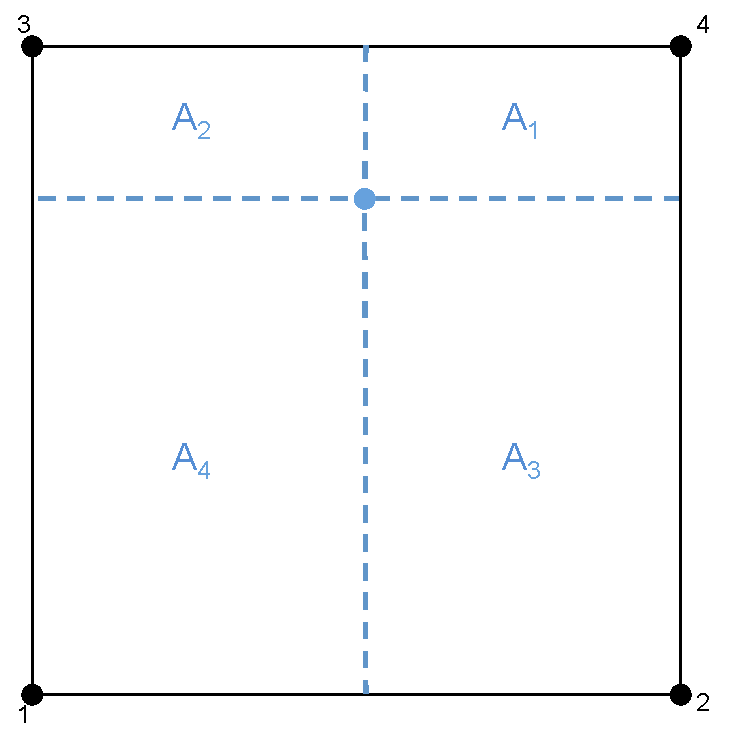
\includegraphics[height=2.5in]{dRdxRVE.pdf}
\end{array}$
\end{center}
\caption{Two-dimensional schematic of $A_i/A$. Blue dot represents fiber node that lies on RVE face. Black dots represent the 4 nodes on an RVE face. The total area of the RVE face is $A=A_1+A_2+A_3+A_4$. }
\label{fig:dRdxRVE}
\end{figure}
%
\subsubsection{Derivative of $V$ with respect to RVE corner coordinates}

The volume can be calculated in the parent domain by
%
\begin{equation}
V = \int_{-1}^{1} \int_{-1}^1 \int_{-1}^1 \text{det}\pmb{J}^e d\xi_1 d\xi_2 d\xi_3  = \int_{-1}^{1} \left(\int_{-1}^1 \left(\int_{-1}^1 \text{det}\pmb{J}^e d\xi_1 \right)d\xi_2\right) d\xi_3 ,
\label{eq:volume}
\end{equation}
%
which has been written in terms of three consecutive integrals. In the biotissue code, the integrals are evaluated using the Gauss integration formula where Eq.\ \eqref{eq:volume} becomes 
%
\begin{equation}
V = \sum_{i=1}^{N_{gp}} \sum_{j=1}^{N_{gp}} \sum_{k=1}^{N_{gp}} W_i W_j W_k \text{det}\pmb{J}^e(\xi_1^{(i)},\xi_2^{(j)},\xi_3^{(k)})
\label{eq:gauss_integration}
\end{equation}
%
where $N_{gp}$ is the number of Gauss integration points, $W_i$ is the weight of the $i^{th}$ integration point, $\pmb{J}^e$ is the Jacobian matrix, and $\xi_i^{(j)}$ is the $i^{th}$ component of the $j^{th}$ integration point. Note that $V$ is the volume for a hexahedron where $N_{gp}=2$, $W_i=1$, and $\xi_i^{(j)}=\pm 1/\sqrt{3}$. 

The derivative of the Volume with respect to the RVE corner coordinates can be written in index notation as
%
\begin{eqnarray}
\frac{\partial V}{\partial x_l^{RVE}} &=& \int_{-1}^1 \int_{-1}^1 \int_{-1}^1 \frac{\partial}{\partial x_l^{RVE}} \left(\text{det}\pmb{J}^e\right) d\xi_1 d\xi_2 d\xi_3 \nonumber\\
%
&=& \sum_{i=1}^{N_{gp}} \sum_{j=1}^{N_{gp}} \sum_{k=1}^{N_{gp}} W_i W_j W_k \frac{\partial}{\partial x_l^{RVE}} \left(\text{det}\pmb{J}^e(\xi_1^{(i)},\xi_2^{(j)},\xi_3^{(k)})\right),
\label{eq:dVdvl}
\end{eqnarray}
%
where we have applied the Gauss integration formula (c.f., Eq.\ \eqref{eq:gauss_integration}). The derivative of det$\pmb{J}^e(\xi_1^{(i)},\xi_2^{(j)},\xi_3^{(k)})$ is 
%
\begin{eqnarray}
&&\frac{\partial}{\partial x_l^{RVE}}\left(\text{det}\pmb{J}^e(\xi_1^{(i)},\xi_2^{(j)},\xi_3^{(k)})\right) \nonumber\\
%
&&= \frac{\partial}{\partial x_l^{RVE}}\bigg[x_{,\xi_1}\left(y_{,\xi_2}z_{,\xi_3} - z_{,\xi_2}y_{,\xi_3} \right) - y_{,\xi_1}\left(x_{,\xi_2}z_{,\xi_3}-z_{,\xi_2}x_{,\xi_3} \right) + z_{,\xi_1}\left(x_{,\xi_2}y_{,\xi_3}-y_{,\xi_2}x_{,\xi_3} \right)\bigg] \bigg |_{\xi_1 = \xi_1^{(i)}, \xi_2 = \xi_2^{(j)}, \xi_3 = \xi_3^{(k)}}.  \nonumber\\
\end{eqnarray}
%
To illustrate, the $x, y, z$ components of the derivative for the ``first" node of the hexahedron $(x_1^{RVE},x_2^{RVE}, x_3^{RVE})$ are explicitly written out:
%
\begin{eqnarray}
\frac{\partial \text{det}\pmb{J}^e}{\partial x_1^{RVE}} &=& \frac{\partial x_{,\xi_1}}{\partial x_1^{RVE}}\left(y_{,\xi_2}z_{,\xi_3} - z_{,\xi_2}y_{,\xi_3} \right) - y_{,\xi_1}\left(\frac{\partial x_{,\xi_2}}{\partial x_1^{RVE}}z_{,\xi_3}-z_{,\xi_2}\frac{\partial x_{,\xi_3}}{\partial x_1^{RVE}} \right) + z_{,\xi_1}\left(x_{,\xi_2}y_{,\xi_3}-y_{,\xi_2}x_{,\xi_3} \right) \nonumber\\
%
&=& \text{det} \begin{bmatrix}
\frac{\partial x_{,\xi_1}}{\partial x_1^{RVE}} & y_{,\xi_1} & z_{,\xi_1} \\
\frac{\partial x_{,\xi_2}}{\partial x_1^{RVE}} & y_{,\xi_2} & z_{,\xi_2} \\
\frac{\partial x_{,\xi_3}}{\partial x_1^{RVE}} & y_{,\xi_3} & z_{,\xi_3}
\end{bmatrix} 
%
= \text{det} \begin{bmatrix}
\frac{\partial N_1^{6\text{hex}}}{\partial \xi_1} & y_{,\xi_1} & z_{,\xi_1} \\
\frac{\partial N_1^{6\text{hex}}}{\partial \xi_2} & y_{,\xi_2} & z_{,\xi_2} \\
\frac{\partial N_1^{6\text{hex}}}{\partial \xi_3} & y_{,\xi_3} & z_{,\xi_3}
\end{bmatrix} \nonumber\\
%%
\frac{\partial \text{det}\pmb{J}^e}{\partial x_2^{RVE}} &=& x_{,\xi_1}\left(\frac{\partial y_{,\xi_2}}{\partial x_2^{RVE}}z_{,\xi_3} - z_{,\xi_2}\frac{\partial y_{,\xi_3}}{\partial x_2^{RVE}} \right) - \frac{\partial y_{,\xi_1}}{\partial x_2^{RVE}}\left(x_{,\xi_2}z_{,\xi_3}-z_{,\xi_2}x_{,\xi_3} \right) + z_{,\xi_1}\left(x_{,\xi_2}\frac{\partial y_{,\xi_3}}{\partial x_2^{RVE}}-\frac{\partial y_{,\xi_2}}{\partial x_2^{RVE}}x_{,\xi_3} \right) \nonumber\\
%
&=& \text{det} \begin{bmatrix}
x_{,\xi_1} & \frac{\partial y_{,\xi_1}}{\partial x_2^{RVE}} & z_{,\xi_1} \\
x_{,\xi_2} & \frac{\partial y_{,\xi_2}}{\partial x_2^{RVE}} & z_{,\xi_2} \\
x_{,\xi_3} & \frac{\partial y_{,\xi_3}}{\partial x_2^{RVE}} & z_{,\xi_3}
\end{bmatrix} 
%
= \text{det} \begin{bmatrix}
x_{,\xi_1} & \frac{\partial N_2^{6\text{hex}}}{\partial \xi_1} & z_{,\xi_1} \\
x_{,\xi_2} & \frac{\partial N_2^{6\text{hex}}}{\partial \xi_2} & z_{,\xi_2} \\
x_{,\xi_3} & \frac{\partial N_2^{6\text{hex}}}{\partial \xi_3} &  z_{,\xi_3}
\end{bmatrix} \nonumber\\
%%
\frac{\partial \text{det}\pmb{J}^e}{\partial x_3^{RVE}} &=& x_{,\xi_1}\left(y_{,\xi_2} \frac{\partial z_{,\xi_3}}{\partial x_3^{RVE}} - \frac{\partial z_{,\xi_2}}{\partial x_3^{RVE}} y_{,\xi_3} \right) - y_{,\xi_1}\left(x_{,\xi_2}\frac{\partial z_{,\xi_3}}{\partial x_3^{RVE}} - \frac{\partial z_{,\xi_2}}{\partial x_3^{RVE}} x_{,\xi_3} \right) + \frac{\partial z_{,\xi_1}}{\partial x_3^{RVE}}\left(x_{,\xi_2}y_{,\xi_3}-y_{,\xi_2}x_{,\xi_3} \right) \nonumber\\
%
&=& \text{det} \begin{bmatrix}
x_{,\xi_1} & y_{,\xi_1} & \frac{\partial z_{,\xi_1}}{\partial x_2^{RVE}}  \\
x_{,\xi_2} & y_{,\xi_2} & \frac{\partial z_{,\xi_2}}{\partial x_2^{RVE}}  \\
x_{,\xi_3} & y_{,\xi_3} & \frac{\partial z_{,\xi_3}}{\partial x_2^{RVE}} 
\end{bmatrix} 
%
= \text{det} \begin{bmatrix}
x_{,\xi_1} & z_{,\xi_1} & \frac{\partial N_3^{6\text{hex}}}{\partial \xi_1}  \\
x_{,\xi_2} & z_{,\xi_2} & \frac{\partial N_3^{6\text{hex}}}{\partial \xi_2}  \\
x_{,\xi_3} & z_{,\xi_3}& \frac{\partial N_3^{6\text{hex}}}{\partial \xi_3} 
\end{bmatrix} .
\label{eq:ddetJdvl}
\end{eqnarray}
%
Note that the formula for the derivatives for each component of the ``second" to ``eighth" nodes of the hexahedron are essentially the same, with the only difference being the shape function: $N_{l}^{6\text{hex}}$ with $l=4$ to $24$ for components corresponding to the second to eighth nodes. The relationship $\partial x_{,\xi_i}/\partial x_j^{RVE} = \partial N_j^{6\text{hex}}/\partial \xi_i$ was used in Eq.\ \eqref{eq:ddetJdvl}.

\subsubsection{Derivative of RVE corner coordinates with respect to finite-element displacements}

The matrix $[\partial \pmb{x}^{RVE}/\partial \pmb{u}^k]$ has dimensions of 24 (8 RVE corner nodes $\times$ 3 dofs per node) $\times$ 12 (4 FE tetrahedron nodes $\times$ 3 dofs per node) for each element: 
%
\setcounter{MaxMatrixCols}{12}
\begin{eqnarray}
\bigg[ \frac{\partial \pmb{x}^{RVE}}{\partial \pmb{u}^k} \bigg] &=& 
\begin{bmatrix}
\frac{\partial x_1^{RVE}}{\partial u_1^k} & \frac{\partial x_1^{RVE}}{\partial u_2^k} & \frac{\partial x_1^{RVE}}{\partial u_3^k} & &
%
 \frac{\partial x_1^{RVE}}{\partial u_{10}^k} & \frac{\partial x_1^{RVE}}{\partial u_{11}^k} & \frac{\partial x_1^{RVE}}{\partial u_{12}^k} \\
%%%
\frac{\partial x_2^{RVE}}{\partial u_1^k} & \frac{\partial x_2^{RVE}}{\partial u_2^k} & \frac{\partial x_2^{RVE}}{\partial u_3^k} & \cdots &
%
\frac{\partial x_2^{RVE}}{\partial u_{10}^k} & \frac{\partial x_2^{RVE}}{\partial u_{11}^k} & \frac{\partial x_2^{RVE}}{\partial u_{12}^k} \\
%%%
\frac{\partial x_3^{RVE}}{\partial u_1^k} & \frac{\partial x_3^{RVE}}{\partial u_2^k} & \frac{\partial x_3^{RVE}}{\partial u_3^k} &  &
%
\frac{\partial x_3^{RVE}}{\partial u_{10}^k} & \frac{\partial x_3^{RVE}}{\partial u_{11}^k} & \frac{\partial x_3^{RVE}}{\partial u_{12}^k} \\
%%%
 & \vdots & & & & \vdots & \\
 %%%
\frac{\partial x_{22}^{RVE}}{\partial u_1^k} & \frac{\partial x_{22}^{RVE}}{\partial u_2^k} & \frac{\partial x_{22}^{RVE}}{\partial u_3^k} & &
%
 \frac{\partial x_{22}^{RVE}}{\partial u_{10}^k} & \frac{\partial x_{22}^{RVE}}{\partial u_{11}^k} & \frac{\partial x_{22}^{RVE}}{\partial u_{12}^k} \\
%%%
\frac{\partial x_{23}^{RVE}}{\partial u_1^k} & \frac{\partial x_{23}^{RVE}}{\partial u_2^k} & \frac{\partial x_{23}^{RVE}}{\partial u_3^k} & \cdots &
%
\frac{\partial x_{23}^{RVE}}{\partial u_{10}^k} & \frac{\partial x_{23}^{RVE}}{\partial u_{11}^k} & \frac{\partial x_{23}^{RVE}}{\partial u_{12}^k} \\
%%%
\frac{\partial x_{24}^{RVE}}{\partial u_1^k} & \frac{\partial x_{24}^{RVE}}{\partial u_2^k} & \frac{\partial x_{24}^{RVE}}{\partial u_3^k} &  &
%
\frac{\partial x_{24}^{RVE}}{\partial u_{10}^k} & \frac{\partial x_{24}^{RVE}}{\partial u_{11}^k} & \frac{\partial x_{24}^{RVE}}{\partial u_{12}^k} \\
\end{bmatrix} \nonumber\\
%
&=&\begin{bmatrix}
\Delta N_1^{(1)} \pmb{I}_{3\times3} & \Delta N_2^{(1)}\pmb{I}_{3\times3} & \Delta N_3^{(1)} \pmb{I}_{3\times3} & \Delta N_4^{(1)}\pmb{I}_{3\times3} \\
%
\Delta N_1^{(2)} \pmb{I}_{3\times3} & \Delta N_2^{(2)}\pmb{I}_{3\times3} & \Delta N_3^{(2)} \pmb{I}_{3\times3} & \Delta N_4^{(2)}\pmb{I}_{3\times3} \\
%
\Delta N_1^{(3)} \pmb{I}_{3\times3} & \Delta N_2^{(3)}\pmb{I}_{3\times3} & \Delta N_3^{(3)} \pmb{I}_{3\times3} & \Delta N_4^{(3)}\pmb{I}_{3\times3} \\
%
\Delta N_1^{(4)} \pmb{I}_{3\times3} & \Delta N_2^{(4)}\pmb{I}_{3\times3} & \Delta N_3^{(4)} \pmb{I}_{3\times3} & \Delta N_4^{(4)}\pmb{I}_{3\times3} \\
%
\Delta N_1^{(5)} \pmb{I}_{3\times3} & \Delta N_2^{(5)}\pmb{I}_{3\times3} & \Delta N_3^{(5)} \pmb{I}_{3\times3} & \Delta N_4^{(5)}\pmb{I}_{3\times3} \\
%
\Delta N_1^{(6)} \pmb{I}_{3\times3} & \Delta N_2^{(6)}\pmb{I}_{3\times3} & \Delta N_3^{(6)} \pmb{I}_{3\times3} & \Delta N_4^{(6)}\pmb{I}_{3\times3} \\
%
\Delta N_1^{(7)} \pmb{I}_{3\times3} & \Delta N_2^{(7)}\pmb{I}_{3\times3} & \Delta N_3^{(7)} \pmb{I}_{3\times3} & \Delta N_4^{(7)}\pmb{I}_{3\times3} \\
%
\Delta N_1^{(8)} \pmb{I}_{3\times3} & \Delta N_2^{(8)}\pmb{I}_{3\times3} & \Delta N_3^{(8)} \pmb{I}_{3\times3} & \Delta N_4^{(8)}\pmb{I}_{3\times3} 
\end{bmatrix},
\label{eq:dRVEdFE_matrix}
\end{eqnarray}
%
where
%
\begin{eqnarray}
\Delta N_j^{(k)} \pmb{I}_{3\times3} &\equiv&
\begin{bmatrix}
\Delta N_j^{(k)} & 0 & 0 \\
0 & \Delta N_j^{(k)} & 0 \\
0 & 0 & \Delta N_j^{(k)} 
\end{bmatrix} \nonumber\\
%
\Delta N_j^{(k)} &\equiv& N_j^{4\text{tet}}(\xi_1^k,\xi_2^k,\xi_3^k) - N_j^{4\text{tet}}(\xi_1^{gp},\xi_2^{gp},\xi_3^{gp}) .
\label{eq:DeltaN_j^k}
\end{eqnarray}
%
In the matrix of Eq.\ \eqref{eq:dRVEdFE_matrix}, each 3 $\times$ 3 submatrix describes the relationship between the degrees of freedom of an RVE corner node and a FE tetrahedron node. These relationships are approximated as 3 $\times$ 3 diagonal matrices where the diagonal terms are calculated as the difference between the $j^{th}$ ($j$ ranges from 1 to 4 for tetrahedron) shape function at the barycentric coordinate of the $k^{th}$ RVE corner-node and that at the barycentric coordinate of the Gauss integration point (c.f., Eq.\ \eqref{eq:DeltaN_j^k}). 

\bibliographystyle{apsrev}
\bibliography{References}
\end{document}